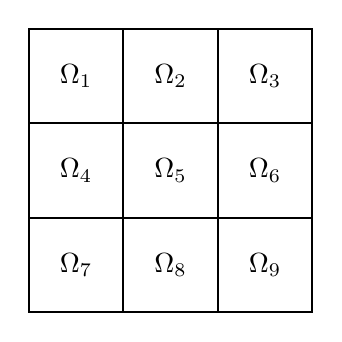
\begin{tikzpicture}[scale=1.2]

% Draw the global square domain
\draw[thick] (0,0) rectangle (3,3);
% \node at (3.3,3.3) {$\Omega$};

% Draw vertical and horizontal grid lines
\foreach \x in {1,2} {
    \draw[thick] (\x,0) -- (\x,3);
    \draw[thick] (0,\x) -- (3,\x);
}

% Label subdomains
\foreach \i in {0,1,2} {
    \foreach \j in {0,1,2} {
        \pgfmathtruncatemacro{\idx}{\i*3 + \j + 1}
        \node at (0.5 + \j, 2.5 - \i) {$\Omega_{\idx}$};
    }
}

\end{tikzpicture}